\subsection{Project structure}

Analysing the requirements of the vehicle helped visualise the four main components of the project: structure, propeller, drivetrain, and pitch control mechanism. A high level of communication was required and, therefore, maintained between the teams working on the different components of the prototype. From the outset of the project, it was planned that the vehicle would be tested experimentally, therefore, planning of the experimental setups began during the later stage of the design process.

Once the designs were complete, manufacturing the drivetrain became an integral part of the project to ensure that the vehicle would be ready for the wind tunnel test. More focus was put on manufacturing to increase progress made on the vehicle before testing. To ensure all aspects of testing were accounted for, an emphasis was put on planning. After deciding on using the wind tunnel facility, a comprehensive plan was laid out for the tests, data collection and data processing.

Once the first wind tunnel test was complete, it was clear that there were still aspects of the vehicle that needed changing prior to the second test. Furthermore, with the overall timescale for the project reducing, it was important to start the analysis of the project outputs. Between wind tunnel tests the focus shifted to improving the vehicle and testing the new features that were implemented.

\subsection{Design Methodology}

\begin{figure}[!htbp]
    \centering
    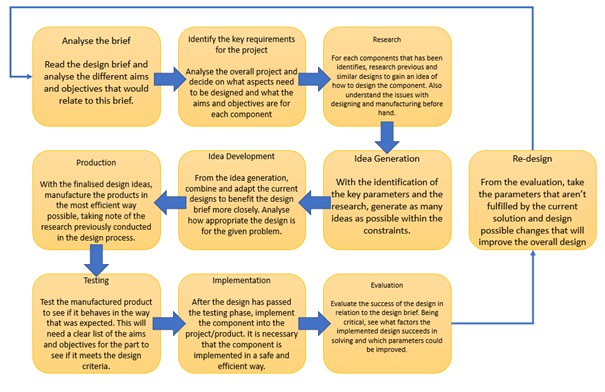
\includegraphics[width=0.7\linewidth]{images/part2/designMethodology.png}
    \caption{Design methodology flow chart}
    \label{fig:desmeth}
\end{figure}

The design methodology for the project focused on employing an iterative method to maximize the outcomes for the vehicle. Following Figure \ref{fig:desmeth} the project was run through this process, ensuring that each stage of design was evaluated properly and that additions to the design were thought out adequately. The project was conducted on a limited budget which enhanced the need to design the vehicle thoughtfully and limit the number of prototypes. Enhancing the vehicle by adding singular improvements sequentially helped reduce the budgetary requirements of the project and reduce overall costs. Working through the structure laid out in Figure \ref{fig:desmeth} was facilitated by the modular nature of the vehicle, as slight improvements could be well thought out before being implementation. Strong communication within the team was important as the performance of the prototype was highly dependent on the synergy between each of its components.

\subsection{Project Timings}

% \begin{figure}[h]
%     \centering
%     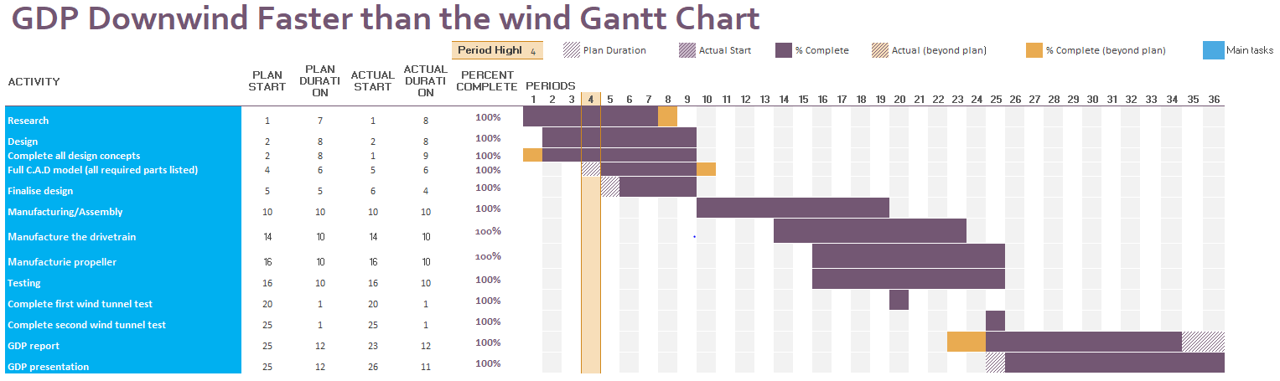
\includegraphics[width=\linewidth] {images/part2/gantt.png}
%     \caption{Gantt chart for project planning}
%     \label{fig:ghantt}
% \end{figure}

This project was run in three main phases: design, manufacture and testing. During the design phase, research was conducted on the various components of the vehicle. This was done in an effort to better understand the workings of the concept as well as maximize the performance of the final output. After research was completed, the information gathered was used in the flow chart of Figure \ref{fig:desmeth} to design the basic vehicle and then iterate through to finalize the project. After completion, the designs were sent to EDMC for manufacturing and finalized post receiving components. The final phase of the project was to test the vehicle, looking at evaluating the performance and understanding the limitations of the design.

\onecolumn
\begin{table}[p]
\caption{Project stakeholders}
\label{tab:stakeholders}
\centering
\begin{tabular}{|
>{\columncolor[HTML]{\CellColor}}l |p{13cm}|p{13cm}|}
\hline
\cellcolor[HTML]{\CellColor} &
  \cellcolor[HTML]{\CellColor}\textbf{Specific   Information Needs} &
  \cellcolor[HTML]{\CellColor}\textbf{Stakeholder   needs and Interests} \\ \cline{2-3} 
\multirow{-2}{*}{\cellcolor[HTML]{\CellColor}\textbf{Project stakeholder name}} &
  \cellcolor[HTML]{\CellColor}\textbf{Types \& Frequency of   Communication} &
  \cellcolor[HTML]{\CellColor}\textbf{Specific areas of interest and participation} \\ \hline
\textbf{Supervisors} &
  Organising weekly meetings with the project supervisors and giving them presentations on the progress of the project in each period was key to the progress of the project. Asking questions and receiving feedback on progress allows for the supervisors to provide detailed analysis and suggestions for improvements for the project. The supervisor's interest in the project is derived from their involvement in the Engineering discipline as researchers at the University &
  This project is derived from the downwind faster than the wind vehicle blackbird created by Rick Cavallaro. The supervisors affect the design of the vehicle directly by inputting their expertise into the project, helping the team understand flaws in their methods \\ \hline
\textbf{Team members} &
  The team members need to stay in contact constantly throughout the project to ensure the project runs   smoothly. Deciding the team roles early on was key for the project as it allowed each team member to know whom to contact with different issues. &
  The team members oversee running the project and ensure the final prototype is up to the standard. The aim is to create a downwind faster than the wind vehicle that runs at the highest speed as is possible. The team were in charge of building the vehicle and will therefore have direct input throughout the project on the design and were the largest contributors affecting the final outcome \\ \hline
\textbf{EDMC} &
  The EDMC team oversaw the manufacturing of all complex components for the vehicle. It was required for the team to stay in contact with the EDMC constantly while parts were being manufactured to ensure that appropriate timescales were upheld for job completion and when they needed any additional information for jobs. &
  The EDMC team were interested in all GDP projects for the university especially in completing project outputs and testing. They have a duty to help each team therefore want to complete all tasks in time as efficiently as possible. Ensuring that the communication was clear was key for this stakeholder as many jobs are submitted to the EDMC throughout the year. This stakeholder has an influence on the design of the project, as over-complicated designs require revision to successfully manufacture components\\ \hline
\textbf{Wind Tunnel team} &
  The main contact for the wind tunnel was David Marshall, the wind tunnel manager. Staying in weekly   contact with him throughout the project was helpful in maintaining a relationship with the facility team and ensuring that all members know the project well, allowing them to help the functionality of test days and achieve better results. &
  The wind tunnel team are interested in the project as the vehicle was run in the RJ Mitchell test   facility. They wanted to ensure that the project didn't damage their wind tunnel, therefore affecting the design by ensuring that the vehicle is safe. They were also interested in the practical outcome of the vehicle due to their involvement in aerodynamic testing. \\ \hline
\textbf{Suppliers} &
  The communication with any possible supplier was held until the components were needed for the vehicle. The frequency of the communications varied depending on the issues that arose from the designing and testing of the vehicle &
  The main interest of the suppliers of components was selling the product to the group. After the components were bought, their interest was directed to the component remaining functional for the buyer. \\ \hline
\end{tabular}
\end{table}
\twocolumn
